% !TeX spellcheck = en_GB

\begin{frame}{Smart Cells}
	\begin{columns}
		
		\begin{column}{0.55\textwidth}
			\begin{tcolorbox}[enhanced jigsaw, colback=white, opacityback=.4, colframe=ElixirPurple, arc=3mm, boxrule=0mm, height=0.8\textheight, valign=center, title=Smart Cell]
				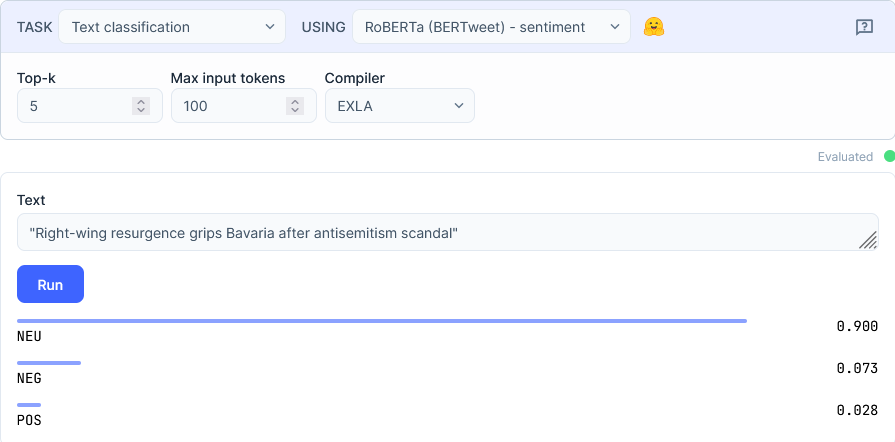
\includegraphics[width=\tcbtextwidth]{pictures/livebook/sentiment_analysis_livebook.png}
			\end{tcolorbox}
		\end{column}
		
		\begin{column}{0.55\textwidth}
			\begin{tcolorbox}[enhanced jigsaw, colback=white, opacityback=.4, colframe=ElixirPurple, arc=3mm, boxrule=0mm, height=0.8\textheight, valign=center, title=Code]
				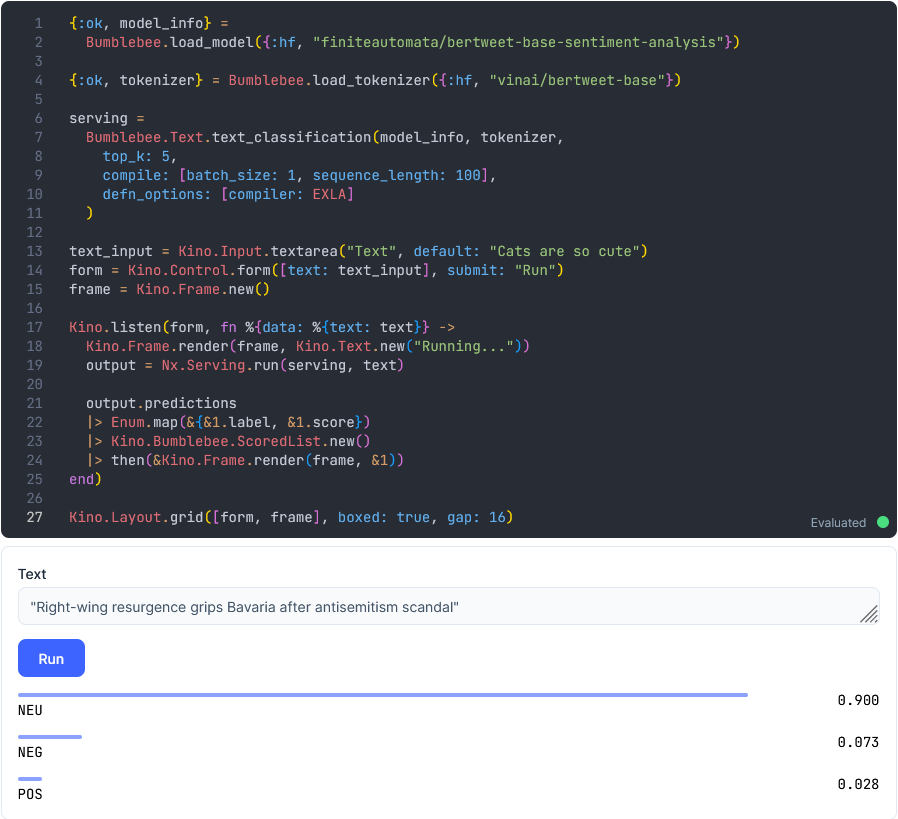
\includegraphics[height=\tcbtextheight]{pictures/livebook/sentiment_analysis_livebook_code.png}
			\end{tcolorbox}
		\end{column}
	\end{columns}
\end{frame}


\begin{frame}[fragile]{Sentiment Analysis English~\footfullcite{perez_pysentimiento_2023}}
\begin{minted}[breaklines, fontsize=\scriptsize]{elixir}
{:ok, model_info} = Bumblebee.load_model({:hf, "finiteautomata/bertweet-base-sentiment-analysis"})
{:ok, tokenizer} = Bumblebee.load_tokenizer({:hf, "vinai/bertweet-base"})

english_sentiment_serving = Bumblebee.Text.text_classification(model_info, tokenizer, compile: [batch_size: 128, sequence_length: 130], defn_options: [compiler: EXLA])

Kino.start_child({Nx.Serving, serving: english_sentiment_serving, name: EngSentimentServer})

english_toots_df = DF.filter(single_party_toots_df, detected_languages == "en")
english_toots = S.to_list(english_toots_df["cleared_content"])
eng_predictions = Nx.Serving.batched_run(EngSentimentServer, english_toots)
\end{minted}
\end{frame}

\begin{frame}[fragile, plain]{Sentiment Analysis German~\footfullcite{guhr_training_2020}}
\begin{minted}[breaklines, fontsize=\scriptsize]{elixir}
{:ok, ger_sent_model_info} = Bumblebee.load_model({:hf, "oliverguhr/german-sentiment-bert"})
{:ok, ger_sent_tokenizer} = Bumblebee.load_tokenizer({:hf, "bert-base-german-cased"})

ger_sent_serving = Bumblebee.Text.text_classification(ger_sent_model_info, ger_sent_tokenizer, compile: [batch_size: 128, sequence_length: 512], defn_options: [compiler: EXLA])

Kino.start_child({Nx.Serving, serving: ger_sent_serving, name: GerSentimentServer})

german_toots_df = DF.filter(single_party_toots_df, detected_languages == "de")
german_toots = S.to_list(german_toots_df["cleared_content"])
ger_predictions = Nx.Serving.batched_run(GerSentimentServer, german_toots)
\end{minted}
\end{frame}

\begin{frame}{Sentiment CSU}
	\begin{figure}[htbp]
		\centering
		\includegraphics[height=0.9\textheight, keepaspectratio]{pictures/paper/sentiments/visualization\_sentiment\_csu.png}
	\end{figure}
\end{frame}



\begin{frame}{Sentiment CSU}
	\begin{figure}[htbp]
		\centering
		\includegraphics[height=0.9\textheight, keepaspectratio]{pictures/paper/sentiments/visualization\_sentiment\_csu.png}
	\end{figure}
\end{frame}


\begin{frame}{Sentiment Frei Waehler}
	\begin{figure}[htbp]
		\centering
		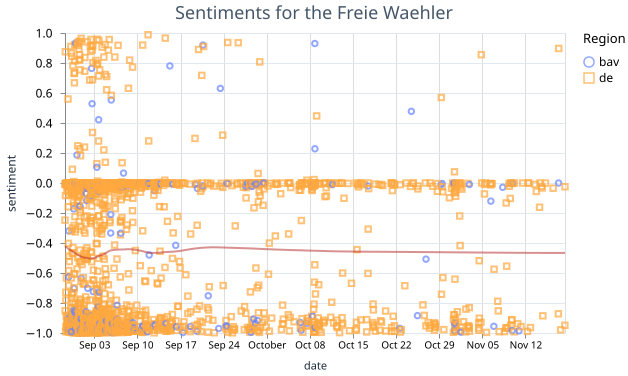
\includegraphics[height=0.9\textheight, keepaspectratio]{pictures/paper/sentiments/visualization_sentiment_fw.png}
	\end{figure}
\end{frame}


\begin{frame}{Sentiment Buendnis 90/Gruene}
	\begin{figure}[htbp]
		\centering
		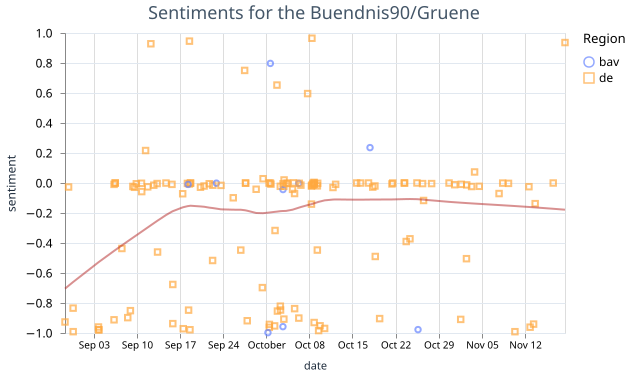
\includegraphics[height=0.9\textheight, keepaspectratio]{pictures/paper/sentiments/visualization_sentiment_gruene.png}
	\end{figure}
\end{frame}
